\subsection{Reconhecimento dos dígitos}
\label{subsec:ocr_desenvolvimento}

O \gls{ocr} implementado divide a leitura em duas etapas: primeiro, localizar no quadro a
janela onde ficam os roletes do hidrômetro; depois, classificar cada dígito dessa janela
separadamente. Os mesmos modelos e a mesma lógica de leitura são usados no
\gls{esp32cam}, no fluxo em borda, e no servidor, no fluxo em nuvem. Esta seção descreve
como essa solução foi escolhida, os dados usados, os dois modelos, a quantização e a forma
de leitura adotada.

\subsubsection{Evolução das abordagens}
\label{subsubsec:evolucao_ocr}

\paragraph{Teste de viabilidade com OCR genérico.}
O primeiro experimento verificou se um \gls{ocr} de propósito geral conseguiria ler o
mostrador em uma imagem tão pequena quanto a capturada pelo \gls{esp32cam}
($160 \times 120$ pixels, em tons de cinza). Em um \textit{notebook} no Google Colab, o
Tesseract 4.1.1 e o EasyOCR 1.7.2 foram aplicados a uma foto do mostrador, cujo valor
visível era \texttt{353485}. Aplicados à linha inteira, nenhum dos dois leu o valor: o
Tesseract devolveu sequências sem sentido, como \texttt{flslalalals}, e o EasyOCR devolveu
\texttt{1581}. A leitura só foi correta quando a imagem foi separada em um recorte por
dígito, por análise de componentes conectados com o OpenCV, e cada recorte foi
reconhecido isoladamente. Por usar uma única foto, o teste serviu apenas como prova de
viabilidade, mas indicou a estrutura adotada: localizar os dígitos e classificá-los um a
um. Os \gls{ocr} genéricos não foram usados nas etapas seguintes.

\paragraph{Pipelines avaliados.}
A partir dessa estrutura, três pipelines de \gls{ocr} foram desenvolvidos em paralelo, e
apenas um foi mantido. A Tabela~\ref{tab:pipelines_ocr} resume os três.

\begin{table}[H]
    \centering
    \caption{Pipelines de \gls{ocr} desenvolvidos}
    \label{tab:pipelines_ocr}
    \begin{tabularx}{\textwidth}{@{}lXXl@{}}
        \toprule
        \textbf{Pipeline} & \textbf{Localização da janela} & \textbf{Leitura dos dígitos} &
        \textbf{Situação} \\
        \midrule
        A & U-Net de $384 \times 384$ pixels, treinada com QAT & CRNN com CTC, lendo a
        janela inteira de uma vez ($48 \times 224$ pixels) & Descartado \\
        B & Rede codificador--decodificador de $192 \times 192$ pixels, INT8 & CNN de um
        dígito ($28 \times 28$ pixels) aplicada a cada rolete & \textbf{Adotado} \\
        C & A mesma U-Net do pipeline A & CNN de um dígito ($68 \times 68$ pixels),
        treinada com dígitos de fontes genéricas & Descartado \\
        \bottomrule
    \end{tabularx}
    \legend{Fonte: Elaborado pelos autores (2026).}
\end{table}

O pipeline A aplicava a arquitetura CRNN com função de perda CTC, apresentada na
Seção~\ref{subsubsec:crnn_ctc}, e foi testado diretamente no \gls{esp32cam}. O teste
mostrou que ele não pode ser executado no microcontrolador: o modelo de localização
exigiu 15.335.424~bytes de memória de trabalho (\textit{arena}) do TensorFlow Lite Micro,
3,8 vezes os cerca de 4~MB de PSRAM da placa, e os modelos de leitura usam o operador
\texttt{REDUCE\_PROD}, ausente na versão da biblioteca disponível no \textit{core}
Arduino-ESP32 3.0.7. O descarte vale para os modelos como foram exportados e não invalida
a abordagem com CTC, que permanece como possibilidade de trabalho futuro. O pipeline C foi
descartado por rodar apenas no computador e por ter o classificador treinado com dígitos
impressos e manuscritos, e não com imagens de hidrômetros. O pipeline B, adotado, é
descrito a seguir.

\subsubsection{Conjuntos de dados}
\label{subsubsec:dados_ocr}

A principal dificuldade para treinar um classificador de dígitos de hidrômetro é a
rotulagem: os conjuntos públicos informam a leitura completa do medidor, e não o valor de
cada rolete. Três fontes de dados foram combinadas, cada uma com um tratamento próprio
para gerar recortes rotulados de um único dígito:

\begin{enumerate}
    \item \textbf{Water Meters Dataset} \cite{kucev2020}: 1.244 fotos de hidrômetros
    variados, tiradas em ângulos arbitrários, com a máscara da janela de dígitos e a
    leitura no nome do arquivo. Foi usado no treinamento do modelo de localização e, para o
    classificador, passou por um processo automático: a janela foi retificada a partir da
    máscara e dividida em células por projeção vertical. Para evitar rótulos errados, só
    foram aceitas as fotos em que a divisão produziu exatamente oito células de larguras
    semelhantes; as demais foram descartadas. Restaram 195 fotos, que geraram 1.560 recortes.
    \item \textbf{Word-Wheel Water Meter Dataset} \cite{zhao2026wordwheel}: conjunto público
    cujo subconjunto de reconhecimento traz recortes padronizados de $200 \times 60$ pixels
    da janela de dígitos, com a leitura completa. Foram descartadas as imagens com um rolete
    no meio da troca entre dois dígitos, cujo rótulo é ambíguo, e as imagens espelhadas
    foram invertidas. Como os recortes já vêm retos, cada um foi dividido em fatias de
    largura igual. Apenas as pastas de treino foram usadas, gerando 47.478 recortes; as
    pastas de teste, com 1.894 imagens, foram reservadas como teste independente.
    \item \textbf{Fotos do próprio \gls{esp32cam}}: para aproximar o modelo das condições
    do sensor, da lente e da compressão do dispositivo, três fotos capturadas pelo
    \gls{esp32cam}, de dois medidores diferentes, tiveram a janela marcada manualmente e
    foram fatiadas e rotuladas à mão, gerando 24 recortes. Esses recortes foram usados
    apenas no ajuste fino (\textit{fine-tuning}) do classificador.
\end{enumerate}

Os dois conjuntos públicos somam 49.038 recortes, com forte desbalanceamento: o dígito 0
tem 20.398 exemplos, pois os roletes mais significativos do medidor costumam marcar zero,
enquanto os demais dígitos têm entre 2.469 e 4.991. Para a validação, a divisão foi feita
por foto, e não por recorte, para que dígitos de uma mesma foto não aparecessem ao mesmo
tempo no treino e na validação: 15\% das fotos foram separadas, resultando em 41.660
recortes de treino e 7.378 de validação.

Uma limitação importante deve ser registrada: as fotos capturadas pelo \gls{esp32cam}
neste trabalho não são de um hidrômetro físico, mas de um monitor que exibia imagens de
hidrômetros. Elas reproduzem o sensor, a lente e a compressão da câmera, mas não os
reflexos no vidro, a iluminação e o ângulo de um medidor instalado.

\subsubsection{Modelo de localização da janela}
\label{subsubsec:segmentacao}

O modelo de localização recebe o quadro redimensionado para $192 \times 192$ pixels e
produz uma máscara binária que indica os pixels da janela de dígitos. Trata-se de uma rede
codificador--decodificador inspirada na U-Net, porém reduzida para caber no
microcontrolador e sem as conexões de salto: duas camadas convolucionais ($3 \times 3$,
com 8 e 16 filtros), cada uma seguida de \textit{max pooling}, duas convoluções transpostas
que restauram a resolução e uma convolução $1 \times 1$ com ativação sigmoide na saída.
Quantizada em INT8, ocupa 11,8~KB.

O modelo foi treinado com o \textit{Water Meters Dataset}, dividido em 70\% para treino,
15\% para validação e 15\% para teste. Como a janela ocupa uma fração pequena da imagem, a
entropia cruzada sozinha levava a rede a classificar quase tudo como fundo; por isso, a
perda adotada combina entropia cruzada e Dice suave, o que elevou o Dice de validação de
0,306 para 0,396 com o mesmo número de épocas. O treino durou 600 épocas, com lotes de 16
imagens, e a melhor época foi a 581. A Figura~\ref{fig:treino_segmentacao} mostra a
evolução do treino.

\begin{figure}[H]
    \centering
    \caption{Evolução do treino do modelo de localização da janela}
    \label{fig:treino_segmentacao}
    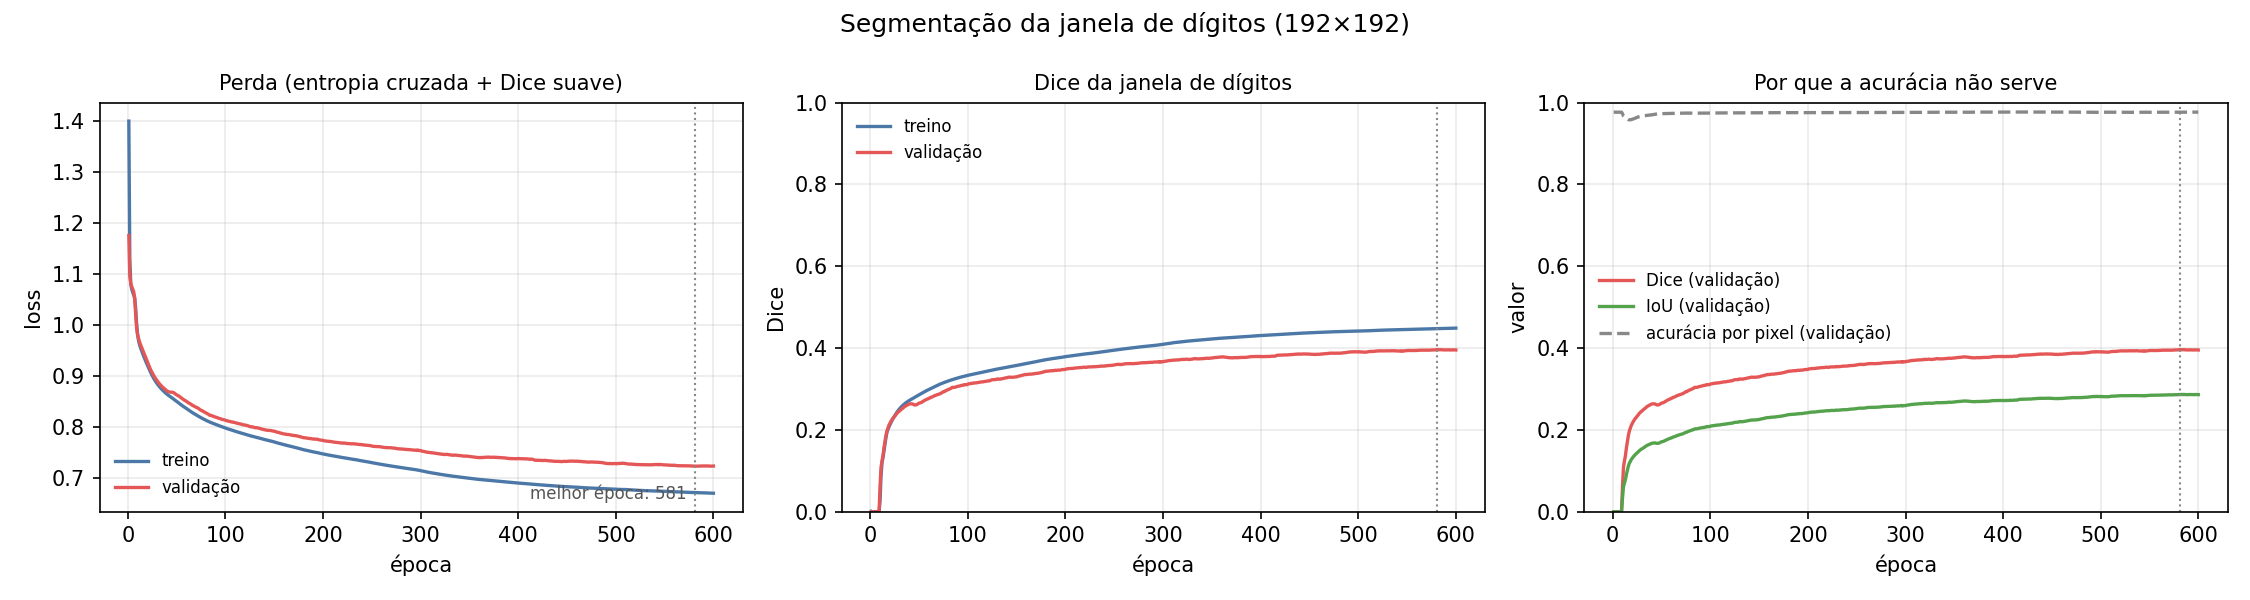
\includegraphics[width=\textwidth]{sections/imagens/ocr_treino_segmentacao.png}
    \legend{Fonte: Elaborado pelos autores (2026).}
\end{figure}

No conjunto de teste, com 186 fotos não vistas no treino, o modelo em INT8 obteve Dice de
0,39 e IoU de 0,28. O resultado é fraco. A acurácia por pixel supera 98\%, mas não serve
como medida, pois o fundo domina a imagem, como mostra o terceiro gráfico da
Figura~\ref{fig:treino_segmentacao}. As curvas de treino e validação próximas indicam
subajuste: a rede, minúscula e sem conexões de salto, não tem capacidade para localizar a
janela com precisão.

No uso, a caixa da janela é o menor retângulo que contém os pixels marcados pela máscara,
convertido para as coordenadas do quadro de $160 \times 120$ pixels. Como a máscara
prevista transborda a janela, essa caixa fica muito maior do que deveria. Nas fotos do
conjunto de teste comum, descrito adiante, a caixa prevista
teve mediana de $125 \times 85$ pixels, cobrindo quase todo o mostrador, enquanto a janela
real mede cerca de $97 \times 18$ pixels. Com essa caixa, cada fatia contém pedaços de
vários roletes e do mostrador, e a leitura falha.

\subsubsection{Classificador de dígitos}
\label{subsubsec:classificador}

O classificador recebe a imagem de um único rolete, redimensionada para $28 \times 28$
pixels em tons de cinza, e devolve a probabilidade de cada um dos dez dígitos. É uma rede
neural convolucional com 72.442 parâmetros, cuja arquitetura é apresentada na
Tabela~\ref{tab:arquitetura_classificador}. Quantizado em INT8, o modelo ocupa 81,5~KB.

\begin{table}[H]
    \centering
    \caption{Arquitetura do classificador de dígitos}
    \label{tab:arquitetura_classificador}
    \begin{tabular}{@{}lll@{}}
        \toprule
        \textbf{Camada} & \textbf{Configuração} & \textbf{Saída} \\
        \midrule
        Entrada & imagem em tons de cinza & $28 \times 28 \times 1$ \\
        Convolução $\times 2$ & 16 filtros $3 \times 3$, ReLU & $28 \times 28 \times 16$ \\
        \textit{Max pooling} & $2 \times 2$ & $14 \times 14 \times 16$ \\
        Convolução $\times 2$ & 32 filtros $3 \times 3$, ReLU & $14 \times 14 \times 32$ \\
        \textit{Max pooling} & $2 \times 2$ & $7 \times 7 \times 32$ \\
        Convolução & 64 filtros $3 \times 3$, ReLU & $7 \times 7 \times 64$ \\
        \textit{Max pooling} & $2 \times 2$ & $3 \times 3 \times 64$ \\
        Achatamento & --- & 576 \\
        Densa & 64 neurônios, ReLU, \textit{dropout} de 30\% & 64 \\
        Densa (saída) & 10 neurônios, \textit{softmax} & 10 \\
        \bottomrule
    \end{tabular}
    \legend{Fonte: Elaborado pelos autores (2026).}
\end{table}

O treinamento foi feito em duas fases. Na fase A, o modelo foi treinado com os recortes dos
dois conjuntos públicos, com o otimizador Adam (taxa de aprendizado de $5 \times 10^{-4}$),
lotes de 128 recortes e pesos por classe para compensar o excesso de zeros. Para aproximar
os recortes das imagens do \gls{esp32cam}, foi aplicado aumento de dados com redução e
ampliação da resolução, ruído gaussiano, pequenas rotações e translações e variação de
contraste. O treino foi interrompido por parada antecipada após 37 épocas, com a melhor
época na 27.ª, e atingiu 94,65\% de acurácia na validação
(Figura~\ref{fig:treino_classificador}).

\begin{figure}[H]
    \centering
    \caption{Evolução do treino do classificador de dígitos (fase A)}
    \label{fig:treino_classificador}
    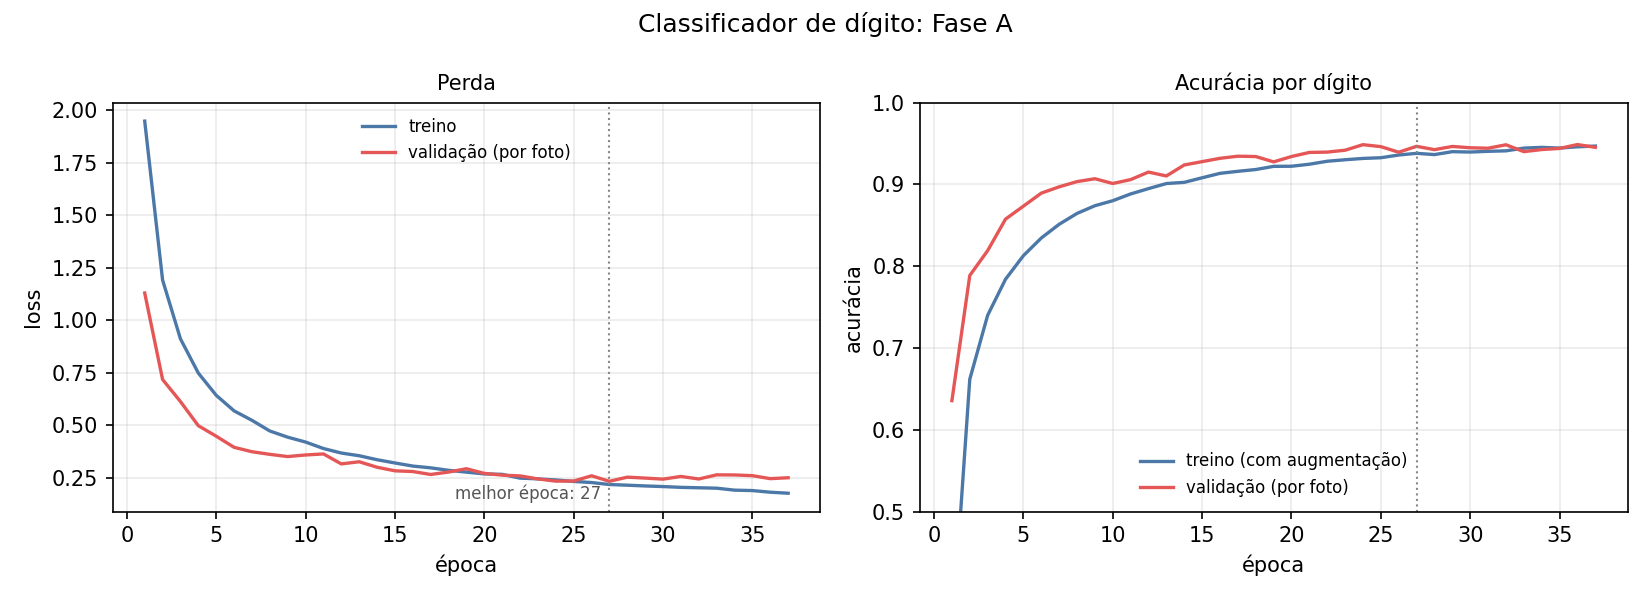
\includegraphics[width=\textwidth]{sections/imagens/ocr_treino_classificador.png}
    \legend{Fonte: Elaborado pelos autores (2026).}
\end{figure}

Na fase B, o modelo passou por um ajuste fino de cinco épocas, com taxa de aprendizado dez
vezes menor ($5 \times 10^{-5}$), usando os 24 recortes do \gls{esp32cam}, fortemente
aumentados e repetidos, junto com uma parte dos recortes da fase A, para que o modelo não
esquecesse o que já havia aprendido. Ao final, a acurácia de validação do modelo em ponto
flutuante foi de 95,46\%.

\subsubsection{Quantização e exportação}
\label{subsubsec:quantizacao_ocr}

Os dois modelos foram quantizados em INT8 após o treinamento (\textit{post-training
quantization}), com um conjunto representativo de imagens para calibrar as escalas. A
quantização foi completa: pesos, ativações, entrada e saída em inteiros de 8 bits, usando
apenas operadores INT8 do TensorFlow Lite. Na entrada, a escala de $1/255$ com ponto zero
de $-128$ permite converter cada pixel diretamente, subtraindo 128 do seu valor. Diferente
do pipeline A, que usou treinamento consciente da quantização (QAT), o pipeline B não
precisou dessa técnica: a perda de acurácia na quantização foi desprezível, como mostra a
avaliação da hipótese H1 nos resultados. Por fim, cada modelo \texttt{.tflite} foi
convertido em um vetor de bytes em um arquivo de cabeçalho C (\texttt{.h}), incluído no
firmware.

\subsubsection{Leitura com janela calibrada na instalação}
\label{subsubsec:leitura_roi}

Dada a caixa da janela, a leitura é feita da mesma forma no firmware e no servidor: a
caixa é dividida em $N$ fatias de largura igual, uma por rolete; cada fatia é
redimensionada para $28 \times 28$ pixels por vizinho mais próximo, convertida para INT8 e
classificada; e os dígitos de maior probabilidade são concatenados na leitura. O número
$N$ de roletes é um parâmetro configurado por medidor: seis no medidor usado nos testes de
hardware.

Como o modelo de localização não encontra a janela com precisão, os resultados com a caixa
prevista por ele são próximos de zero. Esses resultados \textbf{não refletem a capacidade
de leitura do classificador}, e sim o erro da localização: com a caixa errada, as fatias
não correspondem aos roletes. Quando a janela é informada corretamente, o mesmo
classificador lê os dígitos com alta acurácia. A Figura~\ref{fig:leitura_caixa_manual}
mostra cinco capturas do \gls{esp32cam} em que a janela foi marcada à mão: todas as cinco
leituras e os 26 dígitos foram reconhecidos corretamente.

\begin{figure}[htbp]
    \centering
    \caption{Leitura com a janela de dígitos marcada manualmente em cinco capturas do
    \gls{esp32cam}}
    \label{fig:leitura_caixa_manual}
    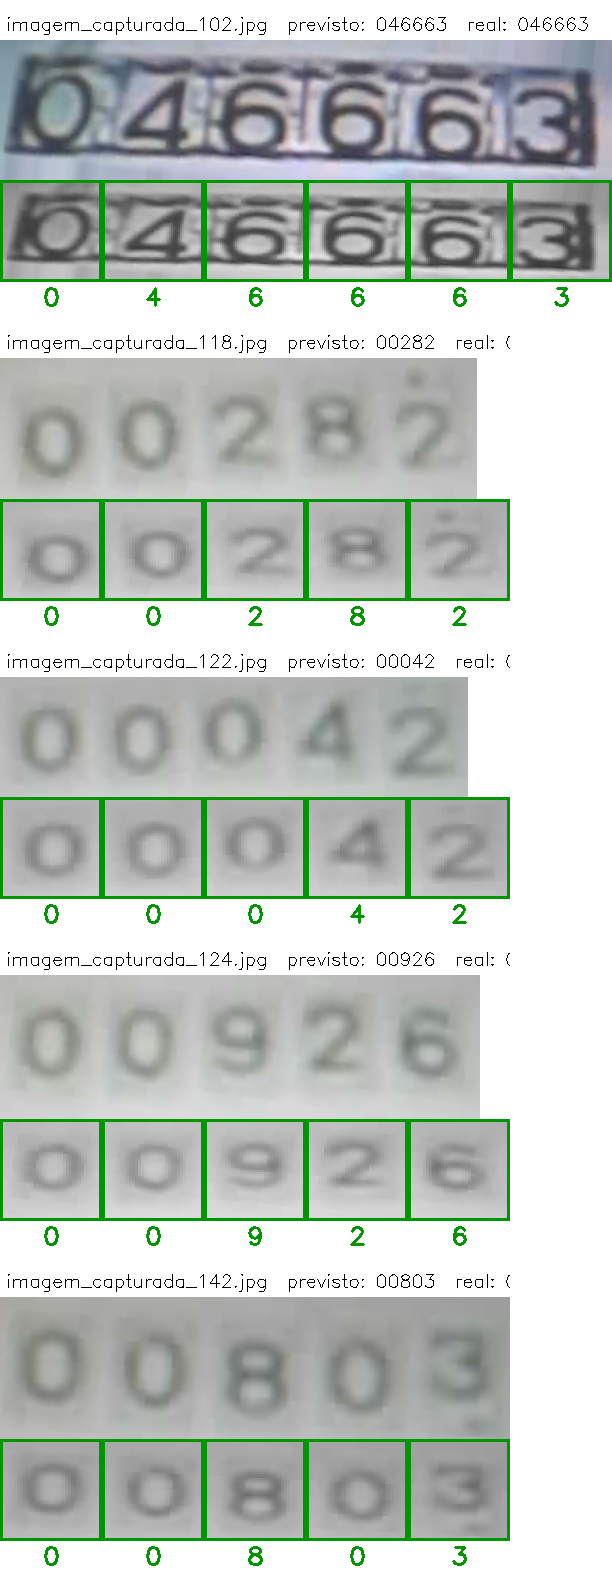
\includegraphics[height=0.55\textheight]{sections/imagens/ocr_leitura_caixa_manual.png}
    \legend{Fonte: Elaborado pelos autores (2026). Em cada captura, a faixa superior é a
    janela recortada, a inferior mostra as fatias e, abaixo, o dígito previsto para cada
    uma.}
\end{figure}

Por isso, a solução adotada dispensa a localização automática. Em uma instalação real, a
câmera fica fixa diante do medidor, de modo que a janela de dígitos ocupa sempre a mesma
região do quadro. Assim, a região de interesse (ROI) e a inclinação dos roletes são
calibradas uma única vez, na instalação, e usadas em todas as leituras seguintes. Essa
calibração precisa ser precisa: a avaliação apresentada nos resultados indica que a ROI
deve estar a cerca de um ou dois pixels da posição correta no quadro de
$160 \times 120$ pixels, em que cada dígito tem aproximadamente 16 pixels de largura.

Nas medições de latência e consumo em hardware, o firmware de borda ainda executava o
modelo de localização a cada leitura, com a câmera posicionada à mão para que a janela
ocupasse a maior parte do quadro e a caixa prevista ficasse próxima dela. Essa configuração é descrita na próxima seção, e o efeito
de remover a localização é discutido nos resultados.
